\begin{table}[t]
\centering
% \def\arraystretch{1.6}
  \begin{tabular}{|c|c|c|c|}
    \hline
    {\multirow{2}{*}{\textbf{Variant}}}  & 
    \multicolumn{2}{c|}{\textbf{Constraints}} & 
    {\multirow{2}{*}{\textbf{Graph connectivity}}}
    % \multicolumn{2}{c|}{\textbf{Graph connectivity}}
    \\
   \cline{2-3}
   &  \textbf{Rest} & \textbf{Activity} &  % & \textbf{Sampling: Guarantee}
\\ \hline
    
A. & \multirow{5}{*}{
     \makecell{ \ref{eq:f0}--\ref{eq:fuse2},\\
     \ref{eq:reach1},\ref{eq:reach2},\\
     \ref{eq:drop1}--\ref{eq:drop4}}
     } 
     & \ref{eq:ann},\ref{eq:aen} & No graph     \\\cline{3-4}
B. & & \ref{eq:anb},\ref{eq:aen} & No graph     \\\cline{3-4}
C. & & \ref{eq:ann},\ref{eq:aeb} & 3-connected  \\\cline{3-4}
D. & & \ref{eq:anb},\ref{eq:aeb} & 2-connected  \\\cline{3-4}
E. & & \ref{eq:ann},\ref{eq:aep} & No graph     \\\cline{3-4}
F. & & \ref{eq:anb},\ref{eq:aep} & 4-connected  \\\hline

% C_es :Self edges are allowed
% C_ed : Every edge is distinct 
  \end{tabular}
\caption{{\bf Activity regulation of molecules vs. graph connectivity.}}
\label{tab:grph}
\end{table}


% Given a system that follows the VTS, we are interested in its connectivity (graph) property.


% The basic idea is to constraint the variables such that vesicular
% transport rules are respected and using constraints (D0-D5) reason
% about the connectivity of the underlying structure (graph).

% We are interested in both least connectivity requirement (LRC) and least guarantee connectivity (LGC).
%LCR, that is required for a vesicular transport version to work and least connectivity that guarantees that vesicular transport system with that connectivity will always satisfies the rules.

% Whether a valid vesicular transport system is of certain connectiviity.   
%negation of the property .... STATE THE MEANING OF RESULT.  

%Besides using the default Z3 solvers we have used for these experiments \ankit{Z3, picoSAT, Lingeling}. The performance of Z3 was ...
%
% \Ankit{In other solver variations ...}

We have implemented the encodings for each variants
using the python interface of $\zthree$ in a tool (MAA).
%
Our tool allows the user to choose a model and the size of the network
besides other parameters like connectivity and number of parallel
edges.
%
It uses Z3 Python interface to build the needed constraints and
applies $\zthree$ solver on the constraints to find a model (
a satisfying assignment that respects the constraints).
%
This tool also translates the satisfying model found by $\zthree$ into
a VTS and presents a visual output to the user in form of annotated graph.
%
% The output graph will satisfy the underlying rules of the system, so
% it always is a valid vesicle transport network.
%
% The resultant graph provides an overview of the underlying VTS
% where directed labeled edges and nodes provide the
% complete information about the system.
%
We also visually report the dropped edges required to disconnect the graph, it gives information about the connectivity of the graph.

% Dashed lines are used in the resultant visual network output to
% specify the dropped edges to make the graph disconnected, which gives
% information about the connectivity of the graph.
%\ashu{discuss table~\ref{tab:grph}}

To illustrate usability of our tool 
in the last column of the table~\ref{tab:grph}, we present the minimum connectedness needed for
the different variants after applying our tool for sizes from 2 to 10. 
%
We found no graph for the variant A with constraints Ann and Aen.
%
Replacing constraint on the node of Ann with Anb (variant B) does not affect the outcome.
%
If we allow every present molecule to stay active (Ann) but constraint the edge
by a boolean function (Aeb) the resultant VTS has to be at least 3-connected. Similarly, the results for the other cases are presented in the table. 
%
% If we constrain the activity of both the edge and the nodes with the boolean function (Anb and Aeb), 
% the VTS has to be 2-connected.
%
We ran experiments varying all parameters for specific N (size). For the comparison between both encodings (Table 2) we have fixed the total number of molecules to be twice as number of the nodes for N $>$ 2 and M = 2N + 1 for N = 2. For each version we also fix total number of parallel edges to maximum two. We have specifically chosen the same connectivity as Table 1 just for illustration purpose; for example in Table~\ref{tab:qf-grabh} Variant A, only check against graph with connectivity 2 is shown, in Variant B with connectivity 3 and similarly for the rest of the Variants. Choice of Variants in the table reflects different type of results variations, for example we left out version B and E as it is of same connectivity type as of A \footnote{Complete result is present in our referenced repository}. 

% Again there is no graph for the case where every molecule on the node is active, but the activity on the edge is driven by pairing inhibition (Aep).
% %
% If we replace the constraint on the node to be a boolean function (Anb) with Aep, we have found that 4-connected graphs satisfies all the constraints.

\begin{table}[t]
  \centering
  \begin{tabular}[t]{|c|c|c|c|c|}\hline
    Size & Model & Connectivity &Formula building (in secs) & Solver (in sec) \\\hline
  \end{tabular}
  \caption{Runtimes for searching for models}
  \label{tab:qf-grabh}
\end{table}
  \todo{Make table for all sizes and variants of the tool}

%--------------------- DO NOT ERASE BELOW THIS LINE --------------------------

%%% Local Variables:
%%% mode: latex
%%% TeX-master: "main"
%%% End:


% In Table~\ref{tab:qf-grabh}, we present the running times for the search of
% VTSs of sizes 2 to 10 that satisfy the variants.
% and compare with our old encoding
% ({Old-e}) from~\cite{shukla}.
% %
% For the comparison between both encodings we have fixed the total
% number of molecules to be $|M| = 2|N|$ for $ |N|> 2$ and
% $|M| = 2|N| + 1$ for $|N| = 2$.
% %
% For each variant, we fix maximum number of parallel
% edges to 2.
% %
% In the table we have shown comparison for specific connectivity, for
% example variant A is checked against any graph with connectivity 2,
% variant B with connectivity 3 similarly for the rest of the Variants.
%
The experiments were done on a machine with Intel(R) Core(TM) i3-4030U
CPU @ 1.90GHz processor and 4GB RAM.
%
We have compared our performance with the performance of our earlier 
CBMC based implementation (old-encoding).
%
For example, the formula for variation F, the total number of
compartments ($|N|$) equals to 10, returns in 129.78 minutes (7786.8 secs)
with a SAT result.
%
In comparison, CBMC results in OUT OF MEMORY for $|N|$ greater than 5.
%
``!'' indicate that the constraints were unsatisfiable.
%
Using this encoding in comparison to the old one, not only we got efficiency improved for finding a SAT model but also did better in the case of refutation that no model exist (Table 2 Variant A timing comparison and Variant D with N =2). Hence with the use of this novel encoding, we are able to scale the system to a much larger compartmentalized system, especially to
eukaryotic cells with a total number of 10 compartments.
%
% \ankit{
% This additional scalability can provide us leverage to ask for related
% open questions that were not previously possible, for example, what is
% the minimum number of molecules required to satisfy the vesicular
% traffic system in eukaryotes.}
%
Furthermore, we experimented with limits of our tools and found
that $\zthree$ was able to solve the constraints up to $\sim{14-18}$ nodes.



% \begin{figure}[t]
  \centering
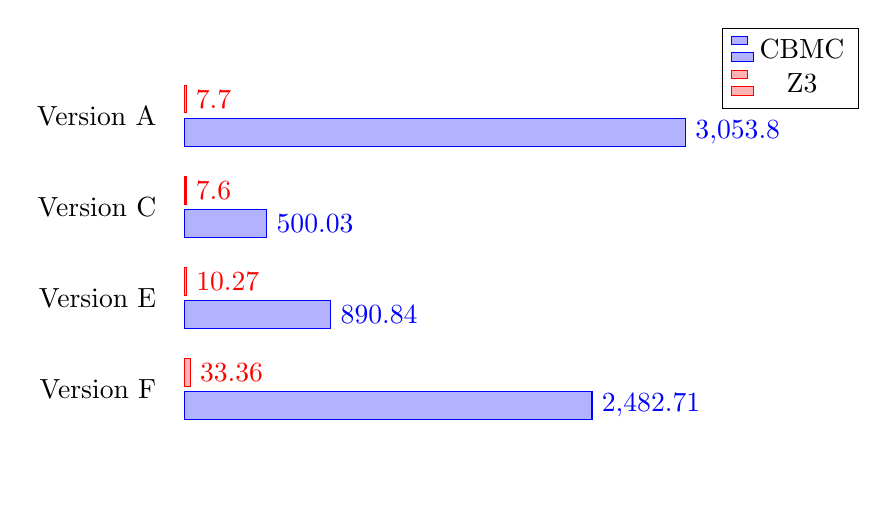
\begin{tikzpicture}
  \begin{axis}[
    xbar,
    y axis line style = { opacity = 0 },
    axis x line       = none,
    tickwidth         = 0pt,
    enlarge y limits  = 0.32,
    enlarge x limits  = 0.04,
    symbolic y coords = {Version F, Version E, Version C, Version A},
    nodes near coords,
    legend pos=outer north east,
  ]
  \legend{CBMC, Z3}
  \addplot coordinates { (3053.8,Version A)         (500.03,Version C)
                         (890.84,Version E)  (2482.71,Version F) };
  \addplot coordinates { (7.7,Version A)         (7.60,Version C)
                         (10.27,Version E)   (33.36,Version F)  };  
  \end{axis}
\end{tikzpicture}  
  \caption{CBMC Vs Z3 encoding for N $\equal$ 5 (in secs)}
  \label{fig:cz-comp}
\end{figure}

%%% Local Variables:
%%% mode: latex
%%% TeX-master: "main"
%%% End:


% REQUIRE COMPARISION WITH CBMC RUN TIME ?

% %
% On this machine, the CBMC encoding ran out of memory (M/O) for N
% $\geq$ 6 whereas new novel encoding was able to handle the case fairly
% easily.
% %
% We think the main reasons for such an improvement are the following:
% \begin{enumerate}
% \item Direct encoding into the solver rather than using CFE (CBMC C front end), which treats front end variables as C variable and similarly other C overheads.
% \item Current novel encoding is fine-tuned to the structure of the problem.
% \item Improved encoding based on reachability rather than complete enumeration and non-determinism.
% \end{enumerate} 
% % 
% %

%table~\ref{tbl:qf-results} 


%--------------------- DO NOT ERASE BELOW THIS LINE --------------------------

%%% Local Variables:
%%% mode: latex
%%% TeX-master: "main"
%%% End:
